\chapter{Validação}

Para validação dos algoritmos foram gerados alguns grafos hipotéticos com cenários distintos.
Muitos deles utilizaram o mesmo vetor de custo, como dito na seção \ref{sec:pathdyn}, que representam
o tempo médio das passagens dos veículos por uma aresta ao longo do dia, em intervalos de 10 minutos.

% \subsection{Cenários de teste}

\subsection{Ferramenta de simulação do caminho mínimo}
Para determinar o caminho mínimo entre dois pontos conhecidos em grafos dinâmicos, foi criado
uma extensão ao Dynagraph, que simula o caminho mínimo. Para isso, segue uma sequência de passos:
\begin{itemize}
\item Ler a estrutura de dados JSON;
\item Exibir o grafo com todos os vértices e arestas;
\item Selecionar um dos 3 algoritmos para exibição do caminho mínimo;
\item Baixar o arquivo JSON, que contém os mesmos dados do grafo mais as arestas do caminho mínimo;
\item Selecionar o dynagraph e abrir o arquivo baixado;
\end{itemize}

As figuras \ref{fig:shortestpath}, \ref{fig:upperlimit} e \ref{fig:downlimit} mostram captura de telas
da ferramenta exibindo exemplos de caminho mínimo dos 3 algoritmos:

\begin{figure}[htbp]
\centering
 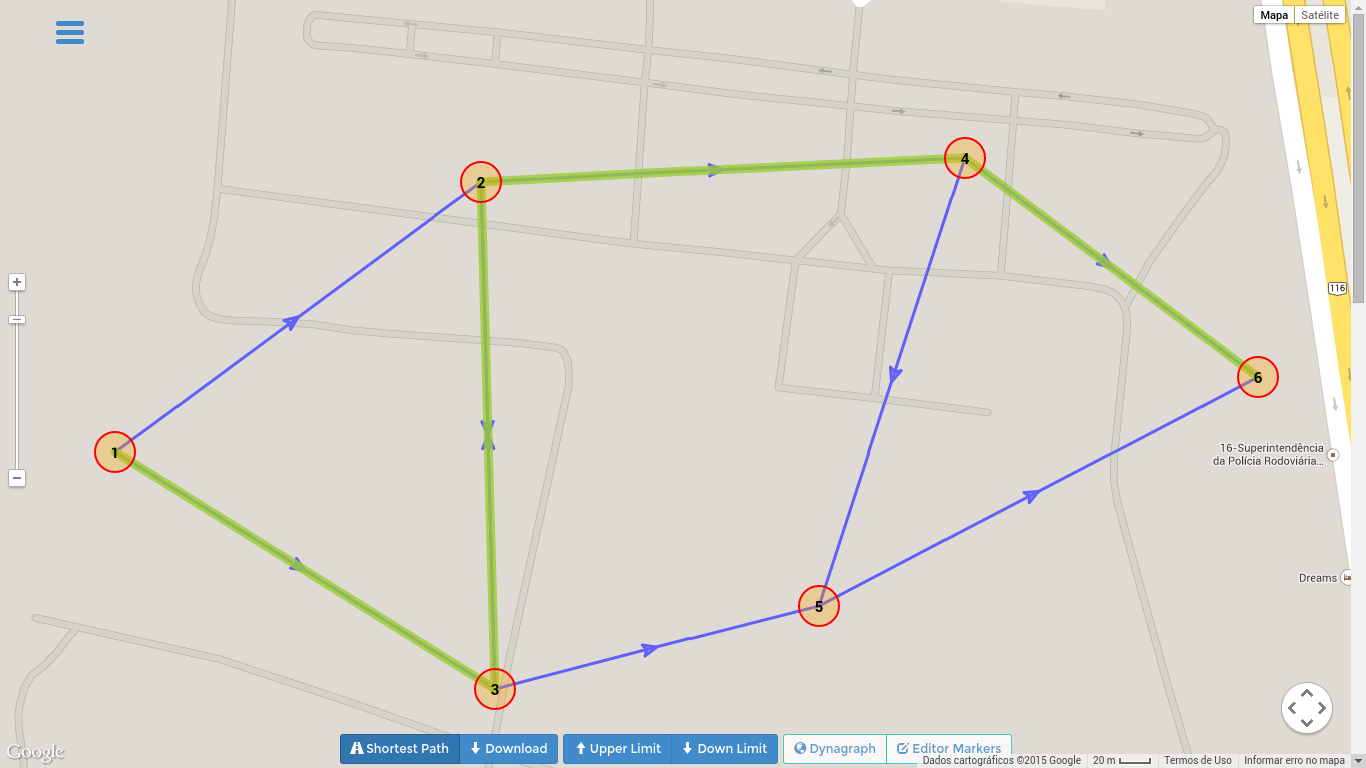
\includegraphics[width=.90\textwidth]{chapters/fig/shortestpath.png}
\caption{Simulador de Caminho Mínimo - Topologia Dinâmica e Atributos Dinâmicos: Limite Superior}
\label{fig:shortestpath}
\end{figure}
\FloatBarrier

\begin{figure}[htbp]
\centering
 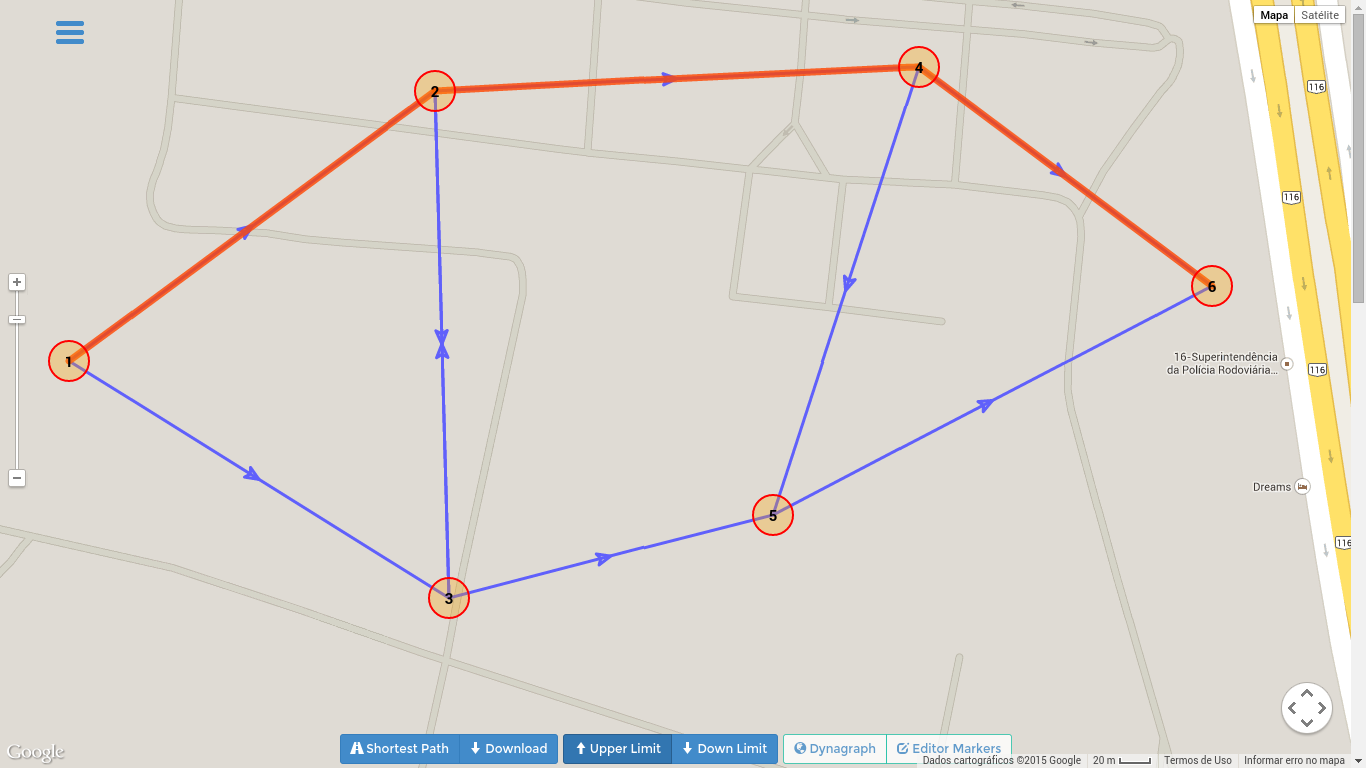
\includegraphics[width=.90\textwidth]{chapters/fig/upperlimit.png}
\caption{Simulador de Caminho Mínimo - Topologia Estática e Atributos Dinâmicos: Limite Superior}
\label{fig:upperlimit}
\end{figure}
\FloatBarrier

\begin{figure}[htbp]
\centering
 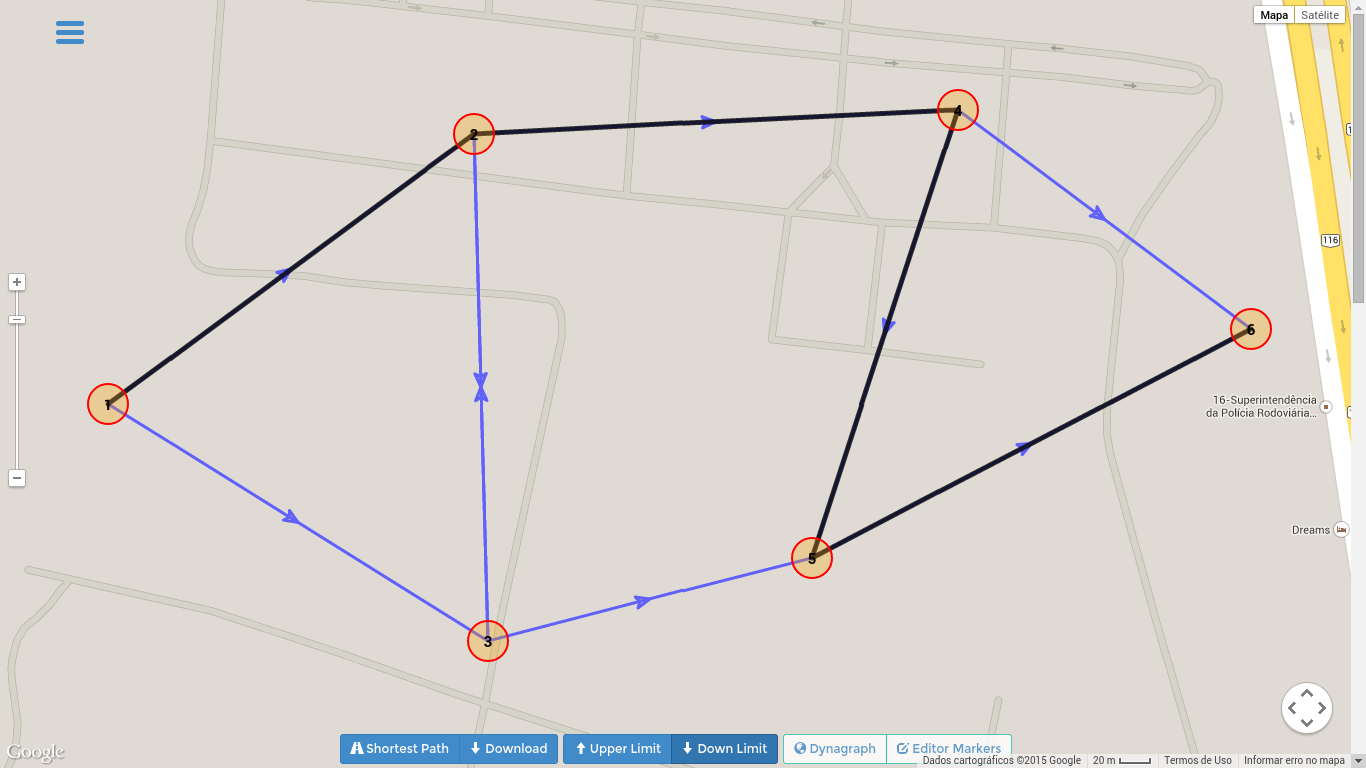
\includegraphics[width=.90\textwidth]{chapters/fig/downlimit.png}
\caption{Simulador de Caminho Mínimo - Topologia estática e Atributos Dinâmicos: Limite Inferior}
\label{fig:downlimit}
\end{figure}
\FloatBarrier

A seguir, serão apresentados os grafos gerados pela ferramenta de simulação com seus respectivos dados.
